\documentclass[12pt,letterpaper]{article}
\usepackage{fullpage}
\usepackage[top=2cm, bottom=4.5cm, left=2.5cm, right=2.5cm]{geometry}
\usepackage{amsmath,amsthm,amsfonts,amssymb,amscd}
\usepackage{lastpage}
\usepackage{enumerate}
\usepackage{fancyhdr}
\usepackage{mathrsfs}
\usepackage{xcolor}
\usepackage{graphicx}
\usepackage{listings}
\usepackage{hyperref}
\usepackage[russian]{babel}

\hypersetup{%
  colorlinks=true,
  linkcolor=blue,
  linkbordercolor={0 0 1}
}
 
\renewcommand\lstlistingname{Algorithm}
\renewcommand\lstlistlistingname{Algorithms}
\def\lstlistingautorefname{Alg.}

\lstdefinestyle{Python}{
    language        = Python,
    frame           = lines, 
    basicstyle      = \footnotesize,
    keywordstyle    = \color{blue},
    stringstyle     = \color{green},
    commentstyle    = \color{red}\ttfamily
}

\setlength{\parindent}{0.0in}
\setlength{\parskip}{0.05in}

% Edit these as appropriate
\newcommand\hwnumber{1}                  % <-- homework number
\newcommand\NetIDa{Rudenko Varvara}           % <-- NetID of person #1


\pagestyle{fancyplain}
\headheight 35pt
\lhead{\NetIDa}
\chead{\textbf{\Large Homework \hwnumber}}
\rhead{ \today}
\lfoot{}
\cfoot{}
\rfoot{\small\thepage}
\headsep 1.5em

\begin{document}

\section{Matrix calculus}
\subsection*{Задача №1}
$\textbf{Find}$ $\bigtriangledown f(x), f(x)= \frac{1}{2} {\left \| Ax-b \right \|}^2_2 , x \in \mathbb{R}^n$

Функцию можно переписать в виде:
$$ f(x)=\frac{1}{2}(Ax-b)^T(Ax-b)$$
Воспользуемся свойством, что $d<x,x>=2<x,dx>$, тогда:
$$ df(x)=\frac{1}{2}d(<Ax-b,Ax-b>)=\frac{1}{2}2<Ax-b,d(Ax-b)>=<Ax-b,Adx>=<A^T(Ax-b),dx>$$
=> $\bigtriangledown f(x)= A^T(Ax-b)$

\subsection*{Задача №2}
$\textbf{Find}\ \triangledown f(X),\ \textbf{if}\ f(X)=<x,x>^{<x,x>}, x\in \mathbb{R}^n\setminus\{0\} $

Сделаем замену $g(x)=<x,x>$, тогда можно переписать функцию $f(x)=g(x)^{g(x)}$. Можем взять градиент от функции и умножить на градиент по самой функции, $d<x,x>=2<x,dx>$, тогда:


\subsection*{Задача №3}
$\textbf{Calculate the Frobenious norm derivative:}\ \dfrac{\partial}{\partial X}||X||_F^2$

По свойству нормы Фробениуса верно, что $ ||X||_F^2 =  \mathbf{tr} \left( X^T X \right) = \mathbf{tr} \left(X X^T \right) = \langle X, X \rangle $, тогда: 
$$
\dfrac{\partial}{\partial X}||X||_F^2 = \dfrac{\partial}{\partial X} \langle X, X \rangle 
$$
По определению производной скалярного произведения:
$$
d ||X||_F^2 = 2 \langle X, d X \rangle =>  \dfrac{\partial}{\partial X}||X||_F^2 = 2 X 
$$

\subsection*{Задача №4}
$\textbf{Calculate the first and the second derivative of the following function}\ f: \textbf{S}\rightarrow\mathbb{R}$
$$f(t)=det(A-tI_n),$$
$\textbf{where}\ A\in\mathbb{R}^{nxn},\ S:=\{t\in\mathbb{R}:det(A-tI_n)\neq0\}. $

Из свойств дифференцирования:
$$
\begin{aligned}
f(t)&=det(A-tI_n)=>df(t)=det(A-tI_n)<(A-tI_n)^{-T},d(A-tI_n)> =\\&=det(A-tI_n)<(A-tI_n)^{-T}(-I_n)^{T},dt)> => \\ &=>f'(t)=det(A-tI_n)(-I_n)^{T}(A-tI_n)^{-T}
\end{aligned}
$$

\subsection*{Задача №5}
Смотри файл autograd.py

\newpage
\section{Convex sets}
\subsection*{Задача №1}
${\textbf{Prove that the set of square symmetric positive definite matrices is convex.}}$

Докажем, что множество является выпуклым конусом. По определению: $ \forall \theta_1, \theta_2 \geqslant 0$ и $ \forall A, B \in \mathbb{S}_{+}^{n} $ 
$$
\theta_{1} A+\theta_{2} B \in \mathbb{S}_{+}^{n}
$$
Матрица, которая получена с помощью такой линейной комбинации остаётся квадратной и симметричной (сумма одинаковых чисел, домноженных на одинаковые константы).\\ 
Матрица положительно определена, по определению $ \forall x \in \mathbb{R}^n $:
$$x^{T}\left(\theta_{1} A+\theta_{2} B\right) x=\theta_{1} x^{T} A x+\theta_{2} x^{T} B x \geq 0$$
так как $A \succeq 0 \rightarrow x^{T} A x \geqslant 0, B \succeq 0 \rightarrow x^{T} B x \geqslant 0  \text { и } \theta_{1}, \theta_{2} \geq 0$\\
По определению - выпуклый конус $=>$ выпуклое.

\subsection*{Задача №2}
$\textbf{Show, that}$ $\textbf{conv}\{xx^T:x\in \textbf{R}^n, \parallel x\parallel =1\}=\{A\in \textbf{S}^n_+: \textbf{tr}(A)=1\}.$


\subsection*{Задача №3}
$\textbf{Show that the hyperbolic set of}$ $ {x \in \mathbb{R}^n_+ | \prod\limits_{i=1}^n x_i \geq 1 } $ $\textbf{is convex. Hint: For}$ $0 \leq \theta \leq 1$ $\textbf{it is valid, that}$ $a^\theta b^{1 - \theta} \leq \theta a + (1-\theta)b$ $\textbf{with non-negative}$ $a,b$.\\

Возьмём такие a и b, чтобы они принадлежали множеству по определению: $ a = \prod\limits_{i} x_{i} \geq 1 \text { и } b = \prod\limits_{i} y_{i} \geq 1 $.
Подставляем в неравенство: 
$$\prod\limits_{i}\left(\theta x_{i}+(1-\theta) y_{i}\right) = \theta \prod\limits_i x_i + \left( 1 - \theta \right) \prod\limits_i y_i  \geq \prod\limits_i x_{i}^{\theta} y_{i}^{1-\theta}=\left(\prod\limits_{i} x_{i}\right)^{\theta}\left(\prod\limits_{i} y_{i}\right)^{1-\theta} \geq 1$$
По определению выпуклого множества, $0 \leq \theta \leq 1$ и $ \forall a, b \in S $, где $ S $ наше множество, выполнено, что $ \theta a + (1 - \theta) b \in S $ => показали выпуклость.

\subsection*{Задача №4}
$\textbf{Prove, that the set}$ $S \subseteq \mathbb{R}^n$ $\textbf{is convex if and only if}$ $(\alpha + \beta)S = \alpha S + \beta S$ $\textbf{for all non-negative}$ $\alpha, \beta$\\

$\blacktriangleright \Rightarrow$ Если $(\alpha + \beta)S = \alpha S + \beta S$ - множество $ S $ выпуклое.
\begin{itemize}
	\item[1) ] По определению, $ \forall x_1, x_2 \in S $ и $ \forall \theta \in [0,1] => \theta x_1 + (1 - \theta) x_2 \in S$
$ \forall x \in \alpha S + \beta S$. \\
Представим в виде: $ x = \alpha z_1 + \beta z_2 $, где $ z_1 \in S \text{и } z_2 \in S$
	\item[2) ] $ x = (\alpha + \beta) z_3$, где $ z_3 \in S $ (так как $(\alpha + \beta)S = \alpha S + \beta S$)\\
Выносим $ \alpha + \beta $ из первого представления:\\
$$ x = \left( \alpha + \beta \right) \left( \frac{\alpha}{\alpha + \beta} z_1 + \frac{\beta}{\alpha + \beta} z_2 \right) \in S $$
	\item[3) ] Получили $ z_3 = \frac{\alpha}{\alpha + \beta} z_1 + \frac{\beta}{\alpha + \beta} z_2  \in S $\\
Заметим, что $ \frac{\alpha}{\alpha + \beta} + \frac{\beta}{\alpha + \beta} = 1$. Пусть $ \theta =  \frac{\alpha}{\alpha + \beta} \Rightarrow  \frac{\beta}{\alpha + \beta} = 1 - \theta$, следовательно:\\
$ z_3 = \theta z_1 + (1 - \theta) z_2  \in S $
Так как $(\alpha + \beta)S = \alpha S + \beta S$ верно для произвольных неотрицательных $ \alpha $ и $ \beta $, то $ \theta = \frac{\alpha}{\alpha + \beta} \in [0,1]. \blacktriangleleft$
\end{itemize}


$\blacktriangleright\Leftarrow S $ - выпуклое множество, доказываем, что $ (\alpha + \beta)S = \alpha S + \beta S $. Доказываем два включения: 
\begin{itemize}
	\item[1) ] $ (\alpha + \beta)S \subseteq \alpha S + \beta S $\\
Возьмём $ z \in (\alpha + \beta)S $ => $ z = (\alpha + \beta)x = \alpha x + \beta x $, где $ x \in S $. Тогда $\forall z \in S $ представим как $ z = \alpha x + \beta x $. Это и есть наше включение: $ (\alpha + \beta)S \subseteq \alpha S + \beta S $
	\item[2) ] $ \alpha S + \beta S \subseteq (\alpha + \beta)S $\\
$ z \in \alpha S + \beta S $, можно представить как: $ z = \alpha z_1 + \beta z_2 $, где $ z_1, z_2 \in S $, можно записать, как $ z = (\alpha + \beta) z_3 $, где $ z_3 \in S $. \\
Как и в доказательстве в другую сторону вынесем скобку $ (\alpha + \beta) $. Получим:\\
$$ z = \left( \alpha + \beta \right) \left( \frac{\alpha}{\alpha + \beta} z_1 + \frac{\beta}{\alpha + \beta} z_2 \right) $$
Снова берём $ \theta = \frac{\alpha}{\alpha + \beta} \Rightarrow \frac{\beta}{\alpha + \beta} = 1 - \theta$ =>
$z = \left( \alpha + \beta \right) \left( \theta z_1 + (1 - \theta) z_2 \right) $\\
$ S $ - выпуклое множество, значит $ \left( \theta z_1 + (1 - \theta) z_2 \right) = z_3 \in S, \forall \theta $\\
Тогда, $ z = \left( \alpha + \beta \right) z_3 \in S $, то есть мы показали обратное включение.\\
\end{itemize}
Доказано, что $ S \text{-выпуклая} \Rightarrow (\alpha + \beta)S = \alpha S + \beta S\blacktriangleleft$

\subsection*{Задача №5}
$\textbf{Let}\ x \in \mathbb{R}\ \textbf{is a random variable with a given probability distribution of}\ \mathbb{P}(x = a_i) = p_i,\ \textbf{where}\ i = 1, \ldots, n, a_1 < \ldots < a_n.\ \textbf{It is said that the probability vector of outcomes of}\ p \in \mathbb{R}^n\ \textbf{belongs to the probabilistic simplex, i.e.}\ P = { p \mid \mathbf{1}^Tp = 1, p \succeq 0 } = { p \mid p_1 + \ldots + p_n = 1, p_i \ge 0 }.\\ \textbf{Determine if the following sets of p are convex:}$

\begin{itemize}
	\item[1) ] $ \mathbb{P}(x > \alpha) \le \beta $\\
В первых трёх пунктах можем сводить к ограничениям на $ p $, как ограничения на полупространство из чего будет следовать, что множество выпуклое.\\
По определению: $ \mathbb{P}(x > \alpha) = \sum\limits_{i: a_i \geqslant \alpha} p_i$, следовательно 
$$
\mathbb{P}(x > \alpha) \le \beta \Leftrightarrow \sum\limits_{i: a_i \geqslant \alpha_i} p_i \le \beta
$$
Геометрически это полупространство и оно выпуклое, значит, наше множество тоже выпуклое.

	\item[2) ] $ \mathbb{E} \vert x^{201}\vert \le \alpha \mathbb{E}\vert x \vert $
По определению матожидания: 
$$
\sum\limits_{i=1}^{n} p_{i}\left(\left|a_{i}^{201}\right|-\alpha\left|a_{i}\right|\right) \leq 0
$$
Не важно, какой коэффициент, главное, чтобы относительно $ p $ было линейное выражение. Можно переписать как $ \sum\limits_{i=1}^{n} c_i p_{i}  $, где $ c_i = \left(\left|a_{i}^{201}\right|-\alpha\left|a_{i}\right|\right) $ - некоторые числовые коэффициенты. Значит, геометрически оно задаёт полупростронство, а оно выпуклое.

	\item[3) ] $ \mathbb{E} \vert x^{2}\vert \ge \alpha  $\\
По опредлению матожидания:
$$ \sum\limits_{i} p_i a_i^2 \geqslant \alpha$$
Тогда из прошлых примеров можем сказать, что оно выпуклое.

	\item[4) ] $ \mathbb{V}x \ge \alpha $\\
По определению дисперсии: 
$$
\mathbb{V}x = \mathbb{E} x^2 - \left( \mathbb{E} x \right)^2 = \sum_{i=1}^{n} a_{i}^{2} p_{i}-\left(\sum_{i=1}^{n} a_{i} p_{i}\right)^{2}=b^{T} p-p^{T} A p \geqslant \alpha
$$
где $ b_{i}=a_{i}^{2} \text { и } A=a a^{T} $ - положительно определённая матрица. Заметим, что такое выражение геометрически задаёт параболу , ветви которой направлены вниз и гиперплоскость $ \alpha $. Нашему множеству принадлежат точки, ограниченные этой гиперплоскостью.
\begin{figure}[h!]
\begin{minipage}[h]{1\linewidth}
\begin{center}
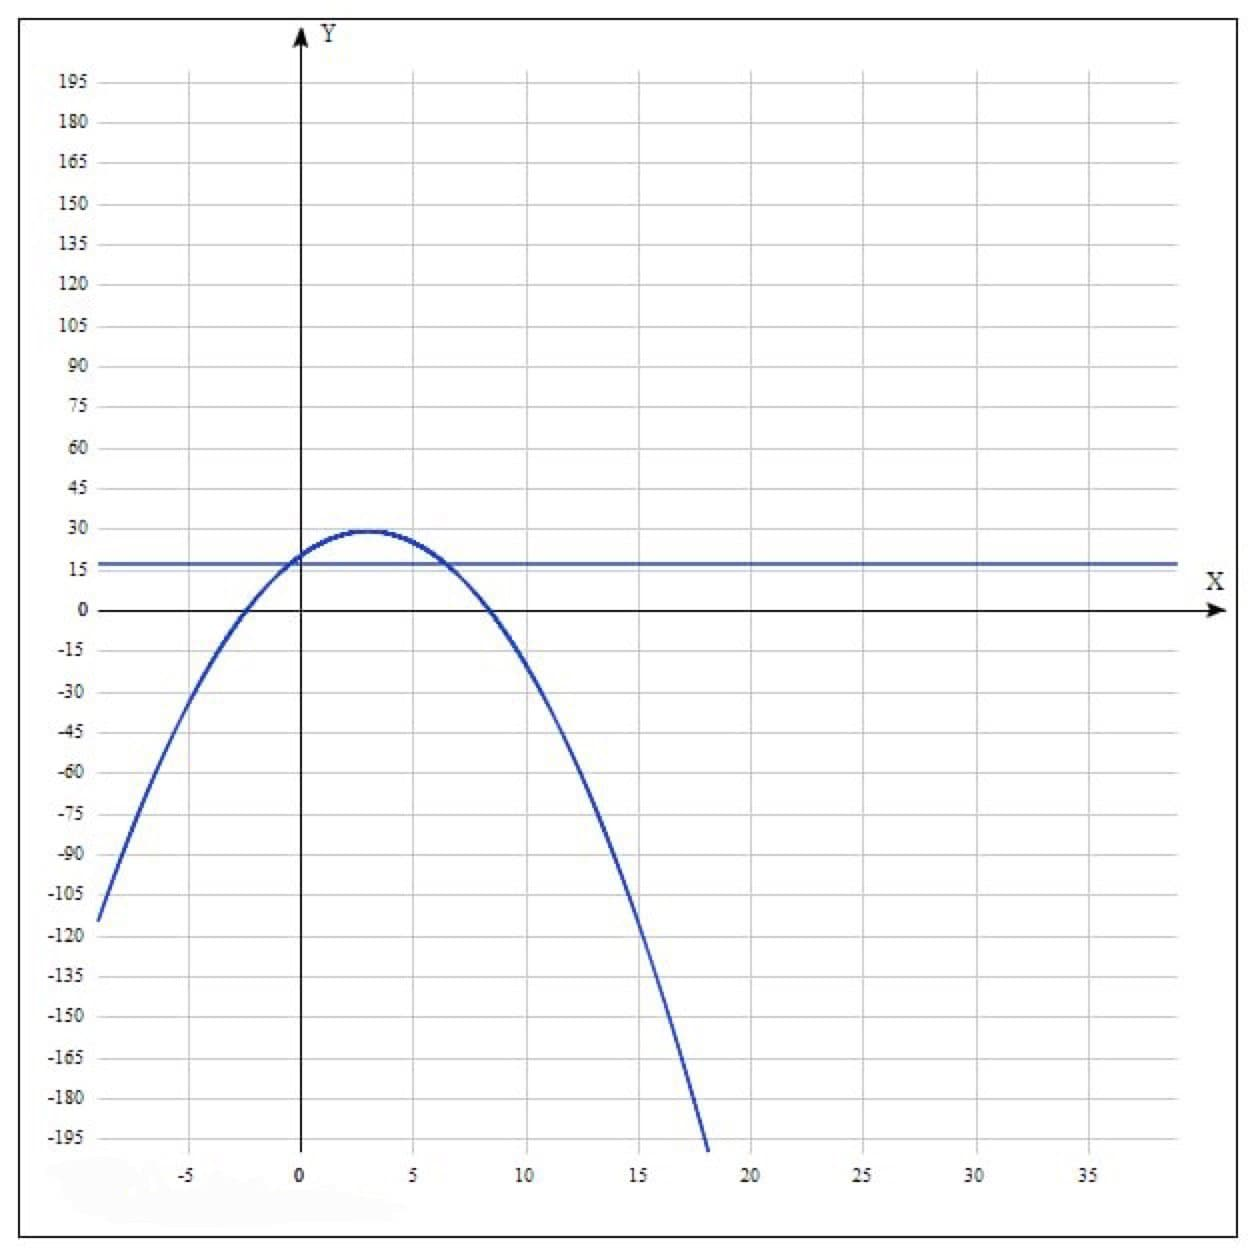
\includegraphics[width=0.6\linewidth]{parab}
\end{center}
\end{minipage}
\end{figure}
Можно утверждать о выпуклости через понятие надграфика: если надграфик функции является выпуклой фигурой, то функция - выпуклая, если выпуклым является подграфик, то функция вогнутая.\\
Перевернутая парабола - вогнутое => подграфик выпуклое множество.
\end{itemize}

\newpage
\section{Convex functions}
\subsection*{Задача №1}
$\textbf{Prove, that function}$ $f(X) = \mathbf{tr}(X^{-1}), X \in S^n_{++}$ $\textbf{is convex, while}$ $g(X) = (\det X)^{1/n}, X \in S^n_{++}$ $\textbf{is concave.}$\\

$\blacktriangleright$ Начнем с доказательства, что $ g(x) $ вогнутая.\\
Функция возвращает скаляр => можем представить как:
$$
g(t)=f(Z+t V), \text { где } Z \succ 0 \text { и } V \in \mathbb{S}^{n}
$$
Получили функцию от скалярной переменной $ t $, которая принимает значения, что $\{t \mid Z+t V \succ 0\}$.
$$
\begin{aligned}
g(t) &=(\operatorname{det}(Z+t V))^{1 / n} \\
&=\left(\operatorname{det} Z^{1 / 2} \operatorname{det}\left(I+t Z^{-1 / 2} V Z^{-1 / 2}\right) \operatorname{det} Z^{1 / 2}\right)^{1 / n} \\
&=(\operatorname{det} Z)^{1 / n}\left(\prod_{i=1}^{n}\left(1+t \lambda_{i}\right)\right)^{1 / n}
\end{aligned}
$$
Где $ \lambda_i $ - собственные числа матрицы $ Z^{-1 / 2} V Z^{-1 / 2} $.\\
Из последнего равенства наша функция $ g(t) $ - вогнута на множестве $\{t \mid Z+t V \succ 0\}$, так как $ \operatorname{det} Z > 0 $, $ Z \succ 0 $ и геометрическое среднее $\prod\limits_{i=1}^{n}\left(x_{i}\right)^{1 / n}$ - вогнуто, а $ 1 + t \lambda_{i} $ - вогнутая функция, то в силу линейности можно говорить, что $ g(X) $ - вогнуто.\\

Для $f(X) = \mathbf{tr}(X^{-1}), X \in S^n_{++}$. Также представим в виде:
$ S (t) = Z + t V $, где $ Z \in S^n_{++} $ и $ V $ - симметрична. Теперь рассматриваем функцию от скалярной переменной $ t $. Достаточно показать (по дифференциальному критерию второго порядка), что для $t=0$
$$  \dfrac {d ^ 2} {dt ^ 2} \mathbf{tr} (S (t) ^ {- 1}) |_{t = 0} \ge 0 $$
Матричное разложение в ряд Тейлора в $t = 0$
$$ S (t) ^ {- 1} = (Z (I + t Z ^ {- 1} V)) ^ {- 1} = Z ^ {- 1} - t Z ^ {- 1} VZ ^ { -1} + t ^ 2 Z^ {- 1} VZ ^ {- 1} VZ ^ {- 1} + \ldots $$ 
поэтому 
$$ \left. \dfrac {d ^ 2} {\partial t ^ 2} \mathbf{tr} (S (t) ^ {- 1}) \right| _ {t = 0} = 2 \mathbf{tr} (Z ^ { -1} VZ ^ {- 1} VZ ^ {- 1}) $$
Но $ Z ^ {- 1} VZ ^ {- 1} VZ ^ {- 1} = UZ ^ {- 1} U ^ T $, где $ U = Z ^ {- 1} V $ и $ Z ^ {- 1 } $ положительно определены (так как $ Z \in S^n_{++} $ и  $ V $ - симметрична), поэтому $ UZ ^ {- 1} U ^ T $ положительно полуопределена, а значит $ \mathbf{tr} (UZ ^ {- 1} U ^ T) \ge 0 $.\\
Следовательно доказали, что $f(X) = \mathbf{tr}(X^{-1})$ - выпуклая функция. $\blacktriangleleft$

\subsection*{Задача №2}
$\textbf{Kullback–Leibler divergence between}$ $p,q \in \mathbb{R}^n_{++}$:
$$ D(p,q) = \sum\limits_{i=1}^n (p_i \log(p_i/q_i) - p_i + q_i) $$
$\textbf{Prove, that}$ $D(p,q) \geq 0 \forall p,q \in \mathbb{R}^n_{++}$, $D(p,q) = 0 \leftrightarrow p = q$\\
$\textbf{Hint:}$ $ D(p,q) = f(p) - f(q) - \nabla f(q)^T(p-q), \quad f(p) = \sum\limits_{i=1}^n p_i \log p_i $

$\blacktriangleright$ По определению дивергенция Кульбака-Лейблера:
$$
D(p, q)=\sum_{i=1}^{n}\left(p_{i} \log \left(p_{i} / q_{i}\right)-p_{i}+q_{i}\right)
$$
$$
D(p, q)=f(p)-f(q)-\nabla f(q)^{T}(p-q), \quad f(p)=\sum_{i=1}^{n} p_{i} \log p_{i}
$$
Тогда: 
$$
\frac{\partial f}{\partial p_{i}}=\log p_i+1
$$
$ \nabla f(p)=\log p+1 $, где $ p $ - вектор. Значит:
$$
D(p, q)=f(p)-f(q)-\nabla f(q)^{T}(p-q) = \sum\limits_ {i=1}^{n} p_i \log p_{i} - q_{i} \log q_{i}-\left(p_{i}-q_{i}\right) \log {q_i} -p_{i}+q_{i}
$$
$$
=\sum\limits_{i=1}^{n}\left(p_i \log p_{i} / q_{i}-p_{i}+q_{i}\right)
$$
Получается определение дивергенции Кульбака-Лейблера.По дифференциальному критерию первого порядка функция выпуклая тогда и только тогда, когда 
$$
f(p) \geqslant f(q) + \nabla f(q)^{T}(p-q) \Leftrightarrow D(p, q)=f(p)-f(q)-\nabla f(q)^{T}(p-q) \geqslant 0
$$
Но функция $ f(p)=\sum_{i=1}^{n} p_{i} \log p_{i} $ - выпуклая, так как это неотрицательная сумма функций $ x \log x $ (задача №6) => $ D(p, q) \geqslant 0 $. \\ Если $ p = q $, то подставив получим $ D(p, q) = 0 \blacktriangleleft$


\subsection*{Задача №3}
$\textbf{Let x be a real variable with the values}$ $ a_1 < a_2 < \ldots < a_n $ $\textbf{with probabilities}$ $ \mathbb{P}(x = a_i) = p_i$. $\textbf{Derive the convexity or concavity of the following functions from p on the set of}$ $\left( p | \sum\limits_{i=1}^n p_i = 1, p_i \geqslant 0 \right) $

\begin{itemize}
	\item[1) ] $\mathbb{E}x$\\
Линейная функция вида $ f(x) c^T x + b $ - выпуклая и вогнутая одновременно (доказывается по определению). По определению матожидания: $$\mathbb{E}x = \sum\limits_{i=1}^n a_i p_i.$$ 
Получили линейную функцию, следовательно, матожидание - выпуклая и вогнутая функция.

	\item[2) ] $\mathbb{P}\{x \geqslant \alpha\}$ \\
Аналогично задаче на множества:
$$\mathbb{P}\{x \geqslant \alpha\} = \sum\limits_{i: a_i \geq \alpha} p_i$$
Получили линейную функцию, следовательно - выпуклая и вогнутая функция.

	\item[3) ] $\mathbb{P}\{\alpha \le x \le \beta\}$\\
Рассматриваем прошлый пункт для другого диапазона:
$$ \mathbb{P}\{\alpha \le x \le \beta\} = \sum\limits_{i: \alpha \le a_i \le \beta} p_i$$
Получили линейную функцию, следовательно - выпуклая и вогнутая функция.

	\item[4) ] $\sum\limits_{i=1}^n p_i \log p_i$\\
В задаче 6 показали, что функция $ x \ln x $ - выпуклая. Тогда наша функция - неотрицательная сумма выпуклых, сепарабельных функций. Тогда получили выпуклую функцию, ведь неотрицательная сумма сохраняет выпуклость.

	\item[5) ] $\mathbb{V}x = \mathbb{E}(x - \mathbb{E}x)^2 = \mathbb{E} x^2 - \left( \mathbb{E} x \right)^2 $\\
Выпуклая функция:
$$f(\theta x+(1-\theta) y) \leq \theta f(x)+(1-\theta) f(y)$$
Существует контрпример $ n = 2, a_1 = 0, a_2 = 1, p_1 = (1, 0), p_2 = (0, 1), \theta = \frac{1}{2} $.
$$ \mathbb{V}(p_1) = \mathbb{E} p_1^2 - \left( \mathbb{E} p_1 \right)^2 = 0$$
$$ \mathbb{V}(p_2) = \mathbb{E} p_2^2 - \left( \mathbb{E} p_2 \right)^2 = 1 - 1 = 0$$
$$ \mathbb{V}(p = (\frac{1}{2}, \frac{1}{2})) = \frac{1}{2} - \frac{1}{4} = \frac{1}{4} $$
$ \frac{1}{4} \nleq 0 $ => дисперсия - вогнутая функция.

	\item[6) ] $\mathbf{quartile}(x) = {\operatorname{inf}}\left( \beta | \mathbb{P}\{x \leqslant \beta\}  \geqslant 0.25 \right)$\\
$\mathbf{quartile}(x)$ не является непрерывной функцией, так как $ x $ может принимать только дискретные значения $ a_1 < a_2 < \ldots < a_n $ => она определена на дискритном множестве точек, которое не является выпуклым. Значит, она не является ни выпуклой, ни вогнутой. 
\end{itemize}

\subsection*{Задача №4}
$\textbf{Is the function returning the arithmetic mean of vector coordinates is a convex one:}$ $a(x) = \frac{1}{n}\sum\limits_{i=1}^n x_i$, $\textbf{what about geometric mean:}$ $g(x) = \prod\limits_{i=1}^n \left(x_i \right)^{1/n}$?\\

$a(x) = \frac{1}{n}\sum\limits_{i=1}^n x_i$ - выпуклая функция. По дифференциальному критерию первого порядка:
$$ a(x+\Delta x) \geq a(x)+\nabla a^{T}(x) \Delta x $$
Градиент берем по координатно, получаем: $ \nabla a^{T}(x) = \left( \frac{1}{n}, \ldots, \frac{1}{n} \right) $. Подставляем в критерий: 
$$ \frac{1}{n} \sum_{i=1}^{n} x_{i}+\frac{1}{n} \sum_{i=1}^{n} \Delta x_{i} \geq \frac{1}{n} \sum_{i=1}^{n} x_{i}+\frac{1}{n} \sum_{i=s}^{n} \Delta x_{i} $$
Это неравенство верно, следовательно, среднее арифмитическое - выпуклая функция.

Геометрическое среднее, которое определяется как: 
$$ g(x)=\prod_{i=1}^{n}\left(x_{i}\right)^{1 / n} $$
является вогнутой функцией. Воспользуемся дифференциальным критерием второго порядка, который звучит так: если мы покажем $\nabla^{2} f(x) \preceq 0 $, то $f(x)$ - вогнутая.\\
Если матрица гессиана отрицательно определена => для любого вектора $ v $, верно 
$$ v^{T} \nabla^{2} f(x) v \leqslant 0 $$
Для начала подсчитаем гессиан. Подсчитаю сначала поэлементно, затем перепишу в матричном виде.\\
Певая производная: 
$$ \frac{\partial}{\partial x_{k}} f(x)=\frac{1}{n}\left(\prod_{i=1}^{n} x_{i}\right)^{\frac{1}{n}-1} \cdot \prod_{i=1 \atop i \neq k}^{n} x_{i} $$

Вторая производная, по этому же элементу: 
$$ \frac{\partial^{2}}{\partial x_{k}^{2}} f(x)=-\frac{n-1}{n^{2}}\left(\prod_{i=1}^{n} x_{i}\right)^{\frac{1}{n}-2} \cdot\left(\prod_{i=1 \atop i \neq k}^{n} x_{i}\right)^{2}=-\frac{n-1}{n^{2}} \times x_k^{\frac{1-2 n}{n}}\left(\prod_{i=1 \atop i \neq k}^{n} x_{i}\right)^{\frac{1}{n}}=  $$
$$= -\frac{n-1}{n^{2} x_{k}^{2}}\left(\prod_{i=1}^{n} x_{i}\right)^{\frac{1}{n}} $$
Получаем, что 
$$ \frac{\partial^{2} f(x)}{\partial x_{k}^{2}}=-(n-1) \frac{\left(\prod_{i=1}^{n} x_{i}\right)^{1 / n}}{n^{2} x_{k}^{2}} $$

Вторая производная по $x_l$, где $ k \neq l $
$$ \frac{\partial^{2} f(x)}{\partial x_{k} \partial x_{l}}=\frac{\left(\prod_{i=1}^{n} x_{i}\right)^{1 / n}}{n^{2} x_{k} x_{l}} $$

$$ \nabla^{2} f(x)=-\frac{\prod_{i=1}^{n} x_{i}^{1 / n}}{n^{2}}\left(n \operatorname{diag}\left(1 / x_{1}^{2}, \ldots, 1 / x_{n}^{2}\right)-a a^{T}\right) $$
где $ a_i = \frac{1}{x_i} $\\
Умножаем гессиан слева и справа на вектор $ v $:
$$ v^{T} \nabla^{2} f(x) v=-\frac{\prod_{i=1}^{n} x_{i}^{1 / n}}{n^{2}}\left(n \sum_{i=1}^{n} v_{i}^{2} / x_{i}^{2}-\left(\sum_{i=1}^{n} v_{i} / x_{i}\right)^{2}\right) \leq 0 $$
и он $ \leq 0 $. Скобки в конце выражения - неравенство Коши-Буняковского, которое звучит как: 
$$ \left(\sum_{i=1}^{n} a_{i}\right)^{2} \leq\left(\sum_{i=1}^{n} 1\right) \sum_{i=1}^{n} a_{i}^{2}=n \sum_{i=1}^{n} a_{i}^{2} $$
Так как $ a_i = \frac{v_i}{x_i}$ => геометрическое среднее - вогнутая функция.

\subsection*{Задача №5}
$\textbf{Is}$ $f(x) = -x \ln x - (1-x) \ln (1-x)$ $\textbf{convex?}$\\

Рассмотрим отдельно $ f(x) = x \ln x $, где $ x $ - скалярная переменная и покажем по дифференциальному критерию второго порядка, что она выпуклая. 
$$ f^{\prime}(x)=\ln x+1, \quad f^{\prime \prime}(x)=1 / x $$
Так как $ x $ стоит под логарифмом, то $ x > 0 $, следовательно, $ f^{\prime \prime}(x) > 0 $. Значит $ f(x) = x \ln x $ строго выпуклая функция. Функция $ g(x) = (1 - x) \ln (1 - x) $ тоже строго выпуклая при $ 1 - x > 0 $.\\
Неотрицательная сумма выпуклых функций сохраняет выпуклость, поэтому\\ $ x \ln x + (1 - x) \ln (1 - x) $ - строго выпуклая функция. Но она стоит с минусом, значит, вогнутая по определению.

\subsection*{Задача №6}
$\textbf{Let}$ $f: \mathbb{R}^n\rightarrow\mathbb{R}$ $\textbf{be the following function:}$
$$f(x)=\sum^k_{i=1}x_{\lfloor i\rfloor},$$
$\textbf{where}$ $1\leqslant k\leqslant n,$ $\textbf{while the symbol}$ $x_{\lfloor i\rfloor}$ $\textbf{stands for the i-th component of sorted}$ $(x_{\lfloor1\rfloor}\textbf{-maximum component of x and} x_{\lfloor n \rfloor}\textbf{-minimum component of x})$ \\ $\textbf{Show, that f is a convex function.}$ 

Можно рассмотреть как максимум различных сумм:
$$ f(x)=\sum^k_{i=1}x_{\lfloor i\rfloor} = max\{x_{i_1}+...+x_{i_r}\mid 1\leq i_1<i_2<...<i_r\leq n\},$$
Тогда можно говорить, что получили поточечный максимум для $\frac{n!}{r!(n-r)!}$ линейных функций. А так как функции линейны, можем сделать вывод, что функция f(x) будет выпуклой.

\newpage
\section{Conjugate sets}
\subsection*{Задача №1}
$\textbf{Let}$ $\mathbb{A}_n$ $\textbf{be the set of all}$ $n$ $\textbf{dimensional antisymmetric matrices. Show that}$ $\left( \mathbb{A}_n\right)^* = \mathbb{S}_n$. \\

Покажем вложения в обе стороны. \\
$\blacktriangleright \left( \mathbb{A}_n\right)^* \subset \mathbb{S}_n  $. Пусть матрица $ B \in \left( \mathbb{A}_n\right)^*, \forall A $ - такой, что $ A^T = -A. $ 
$$ tr \left( A^T B \right) = tr \left( A B^T \right) \geq -1  $$
Пользуясь тем, что $ A^T = -A $:
$$ tr \left( -AB \right) \geq -1 $$
$$ tr \left( A B^T \right) \geq -1$$
Складываем эти 2 неравенства:
$$ tr \left( A \cdot (B^T-B) \right) \geq -2 $$
$$
tr \left( A \cdot (B- B^T) \right) \leq 2
$$
Матрица $ B \in  \mathbb{S}_n $, то есть $ B = B^T $. Доказательство от противного: \\
Пусть $ B \neq B^T $ диагональ не меняется при транспонировании, значит, если вычесть эти матрицы - получим все 0 и хотя бы один ненулевой элемент. Матрица А была взята такой, чтобы у нее на диагонали были нули. Выбираем элементы так, чтобы на диагонали у матрицы $ A (B-B^T) $ был хотя бы 1 элемент.\\ 
Можем это сделать всегда: пусть ненулевой элемент у матрицы $ (B-B^T) $ будет в первом столбце: $ b_{i1} $ ($i\neq1$). Тогда в первой строке матрицы $A$ выбираем $ a_{1i} \neq 0 $ а остальные равные нулю. При произведении получим ненулевой элемент на диагонали $ c = b_{i1} \cdot a_{1i}  $.\\
След матрицы равен сумме диагональных  элементов. Пусть у $ (B-B^T) $ только 1 ненулевой элемент, значит  $ tr \left( A \cdot (B- B^T) \right) = c$. Так как матрица $ A $ произвольная, то можем взять её с элементом  $a_{1i} \cdot \frac{3}{c} $. Тогда $ tr \left( A \cdot (B- B^T) \right) = 3 > 2 $ получаем противоречие, что $ B \in \left( \mathbb{A}_n\right)^* $.\\ 

Если в матрице $ (B-B^T) $ > 1 ненулевого элемента, нельзя доказать, что след равен 0: \\
матрица $ (B-B^T) $ - антисимметричная, для произвольной антисимметричной матрицы $ B^* =  (B-B^T) $ можно подобрать такую антисимметричную $ A $, что $ tr (A B^*) \neq 0$. Просто будем брать такую же и получаем отрицательно определённую (на диагонале будут стоять числа одного знака и след не занулится), применяем рассуждения для одного ненулевого элемента - и получаем противоречие. Значит, $ B = B^T $, $ B \in \mathbb{S}_n \rightarrow \left( \mathbb{A}_n\right)^* \subset \mathbb{S}_n \blacktriangleleft$\\

$\blacktriangleright$ Вложение в другую сторону: пусть $ B \in \mathbb{S}_n $, то есть $ B = B^T $ а $ A $ - произвольная антисимметричная матрица, тогда: 
$$
tr (A B^T) = tr(AB) 
$$
$$
tr(A^T B) = - tr (AB)
$$
Получается, что $ tr(AB)=-tr(AB) \rightarrow tr(AB) = 0 > -1 $, значит $ B \in \left( \mathbb{A}_n\right)^* \rightarrow \left( \mathbb{A}_n\right)^* \supseteq \mathbb{S}_n$\\
Получаем, что $\left( \mathbb{A}_n\right)^* = \mathbb{S}_n \blacktriangleleft$


\subsection*{Задача №2}
$\textbf{Find the conjugate set to the ellipsoid:}$ 
$$
S = \left\{ x \in \mathbb{R}^n \mid \sum\limits_{i = 1}^n a_i^2 x_i^2 \le \varepsilon^2 \right\}
$$

Определение конуса через матрицу: 

$$
S = \left\{ x \in \mathbb{R}^n \mid \sum\limits_{i = 1}^n \left( \frac{a_i}{\varepsilon} \right) ^2  x_i^2 \le 1 \right\}
$$

$ A = \operatorname{diag} (\frac{a_i}{\varepsilon}) $ - диагональная матрица, тогда $$ \| Ax \|_2^2 = 
 \sum\limits_{i = 1}^n \left( \frac{a_i}{\varepsilon} \right) ^2  x_i^2 $$
 
Задаем эллипс:
$$
S = \left\{ x \in \mathbb{R}^n \mid \| Ax \|_2  \le 1 \right\} =E= \left\{ A^{-1}u \mid \| u \|_2  \le 1 \right\}\ \text{(Бойд)} 
$$
Где $A^{-1}=diag\frac{\varepsilon}{a_i}$. Что эквивалентно, покажем через вложение множеств одно в другое:\\
$2\rightarrow1$: $ x = A^{-1}u $, где $ \| u \|_2  \le 1 $, подставим в S, тогда $  \|  A A^{-1}u \|_2  \le 1 $ - следовательно, $ E \subseteq S $\\
$2\rightarrow1$: $ \| Ax \|_2  \le 1 $, обозначим $ y = Ax $, получается, что $ \| y \|_2  \le 1 $. Тогда $ x = A^{-1}y $, где $ \| y \|_2  \le 1 $, следовательно $ x \in E $ и $ S \subseteq E $\\

По определению хотим найти все векторы $ p \in E^* $, что $ \forall x \in E \rightarrow \langle p, x \rangle \geq -1$. Любой вектор $ x \in E $ представим как $ x = A^{-1}u $, где $ \| u \|_2  \le 1 $, => для p:
$$
\langle p, A^{-1} u \rangle \geq -1, \; \text{где } \| u \|_2  \le 1
$$
$$
\langle A^{-T} p,  u \rangle \geq -1, \; \text{где } \| u \|_2  \le 1
$$

Из неравенства Коши-Буняковского:
$$
| \langle A^{-T} p,  u \rangle | \leq \| u \|_2 \cdot \| A^{-T} p \|_2 \leq \left[ \| u \|_2 \leq 1 \right] \leq \| A^{-T} p \|_2
$$

Так как вектор $ u $ - произвольный, то равенство может достигаться всегда, поэтому нам подходят все $ p $, для которых выполнено:
$$
-1 \leq - \| A^{-T} p \|_2 \Leftrightarrow \| A^{-T} p \|_2 \leq 1
$$
Такоенеравенство задает эллипс с другой матрицей $ A^{-T} = \operatorname{diag} (\frac{\varepsilon}{a_i})$. Или в привычном виде:

$$
E^* = \left\{ x \in \mathbb{R}^n \mid \sum\limits_{i = 1}^n \left( \frac{\varepsilon}{a_i} \right) ^2  x_i^2 \le 1 \right\}
$$
что эквивалентно
$$
E^* = \left\{ x \in \mathbb{R}^n \mid \sum\limits_{i = 1}^n \left( \frac{1}{a_i} \right) ^2  x_i^2 \le \left( \frac{1}{\varepsilon} \right)^2 \right\}
$$

\subsection*{Задача №3}
$\textbf{Find the sets}\ S^{*}, S^{**}, S^{***}$,     
$$
S = \{ x \in \mathbb{R}^2 \mid x_1 + x_2 \ge 0, \;\; 2x_1 + x_2 \ge -4, \;\; -2x_1 + x_2 \ge -4\}
$$

$ S $ - замкнуто, выпукло и включает 0, то $ S^{**} = S $, $ S^{***} = S^{*} $. Смотрим на рисунках, что это верно:\\
Изображаем $ S $:
\begin{figure}[h!]
\begin{minipage}[h]{1\linewidth}
\begin{center}
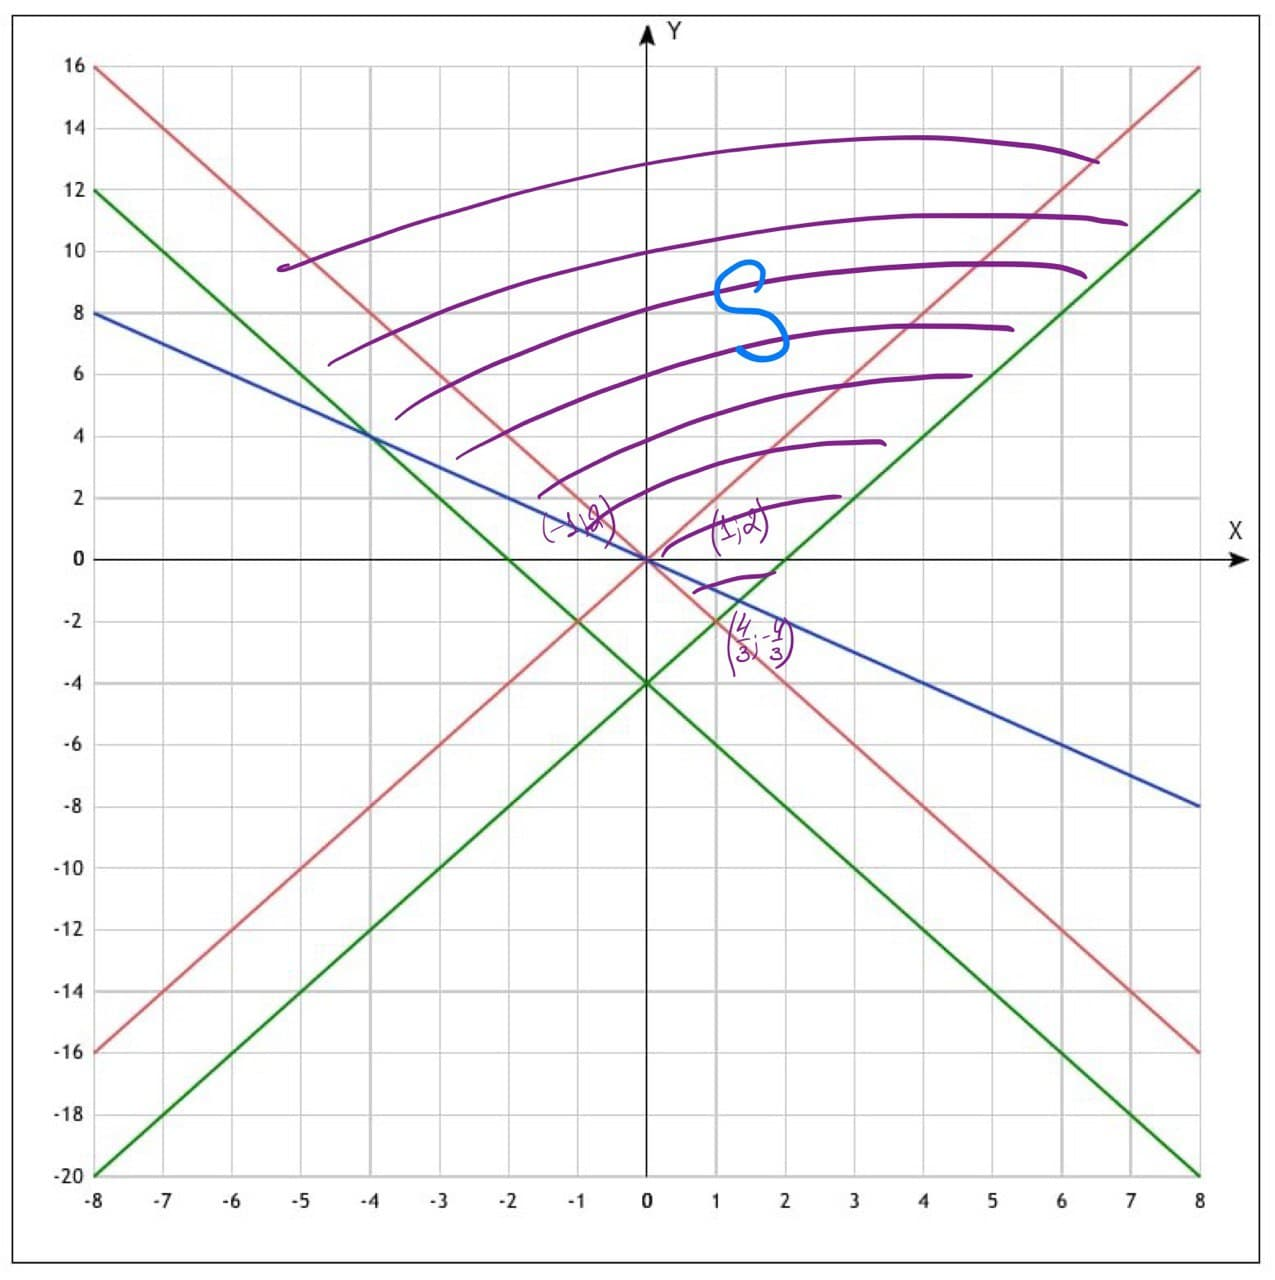
\includegraphics[width=0.6\linewidth]{S}
\end{center}
\end{minipage}
\end{figure}

$$
S=\operatorname{conv}\left((-4, 4), (\frac{4}{3}, -\frac{4}{3}) \right)+\operatorname{cone}\left((1,2), (-1, 2) \right)
$$
\newpage
Получаем следующие неравенства: 
$$
\left\{\begin{array}{c}
-4 p^{1}+4 p^{2} \geq-1 \\
4 p^{1}-4 p^{2} \geq-3 \\
p^{1}+2 p^{2} \geq 0 \\
-p^{1}+2 p^{2} \geq 0
\end{array}\right.
$$

Изобразим $ S^* $:
\begin{figure}[h!]
\begin{minipage}[h]{1\linewidth}
\begin{center}
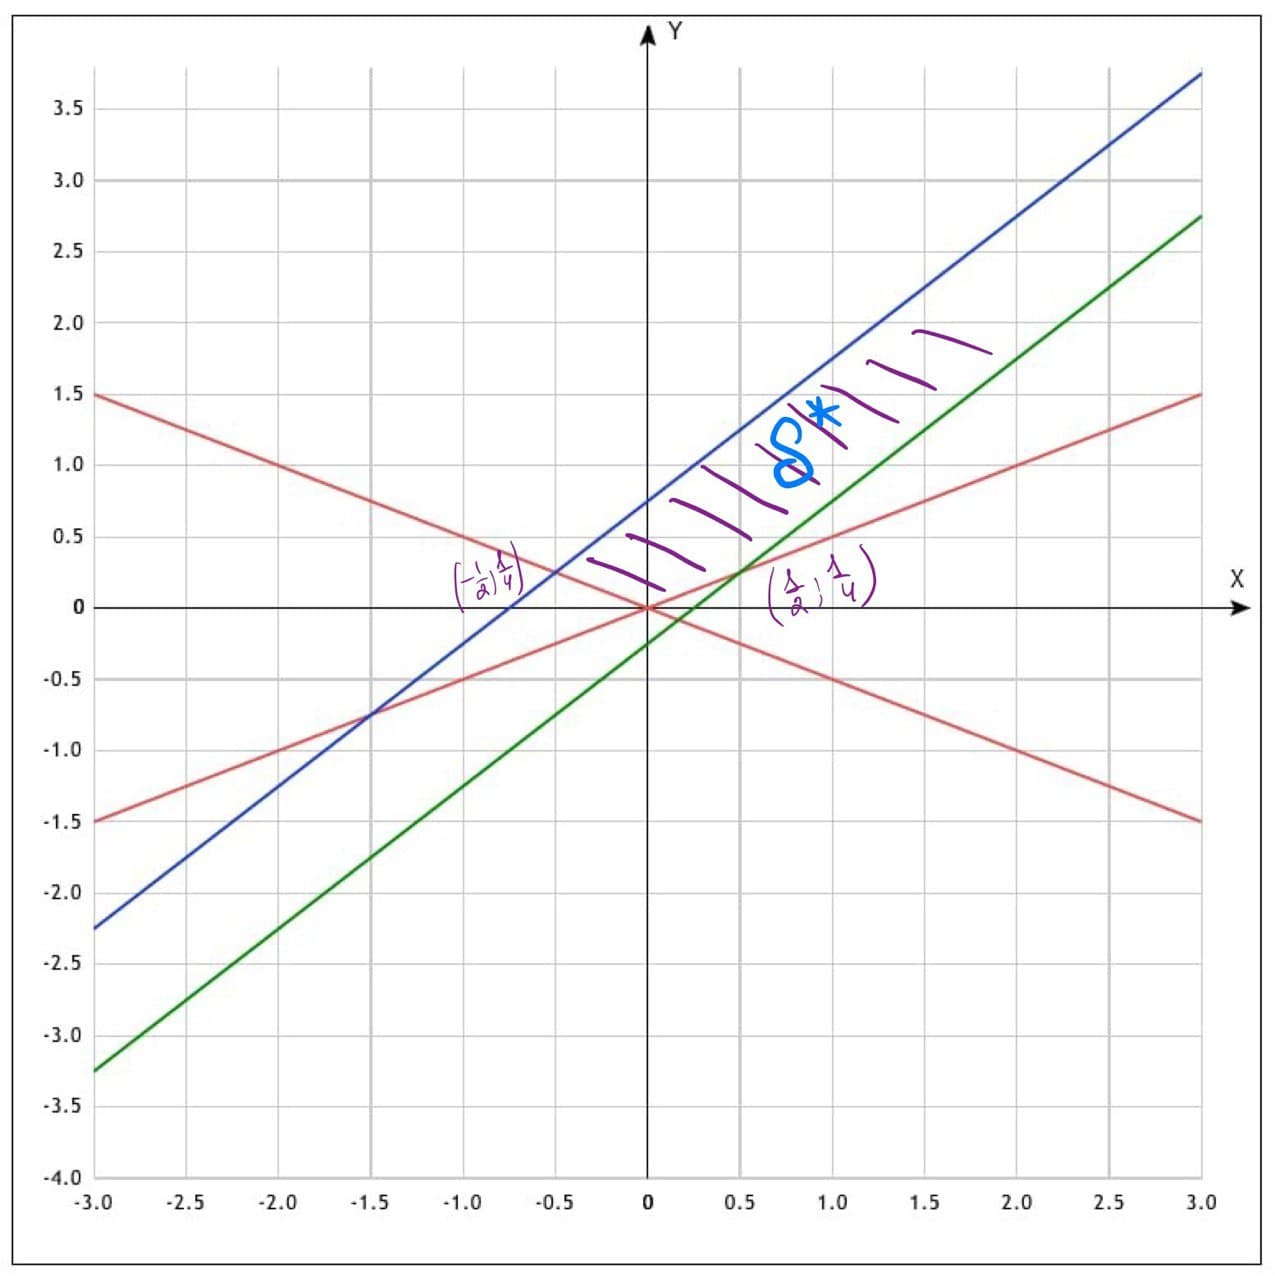
\includegraphics[width=0.6\linewidth]{S2}
\end{center}
\end{minipage}
\end{figure}
 
$$
S^*=\operatorname{conv}\left(\left(-\frac{1}{2}, \frac{1}{4} \right), \left( 0,0 \right),  \left( \frac{1}{2}, \frac{1}{4} \right) \right)+\operatorname{cone}\left((1,1) \right)
$$

\newpage
$$
\left\{\begin{array}{l}
-2 p^{1}+p^{2} \geq-4 \\
2 p^{1}+p^{2} \geq-4 \\
p^{1}+p^{2} \geq 0
\end{array}\right.
$$

Изобразим $ S^{**} $:
\begin{figure}[h!]
\begin{minipage}[h]{1\linewidth}
\begin{center}
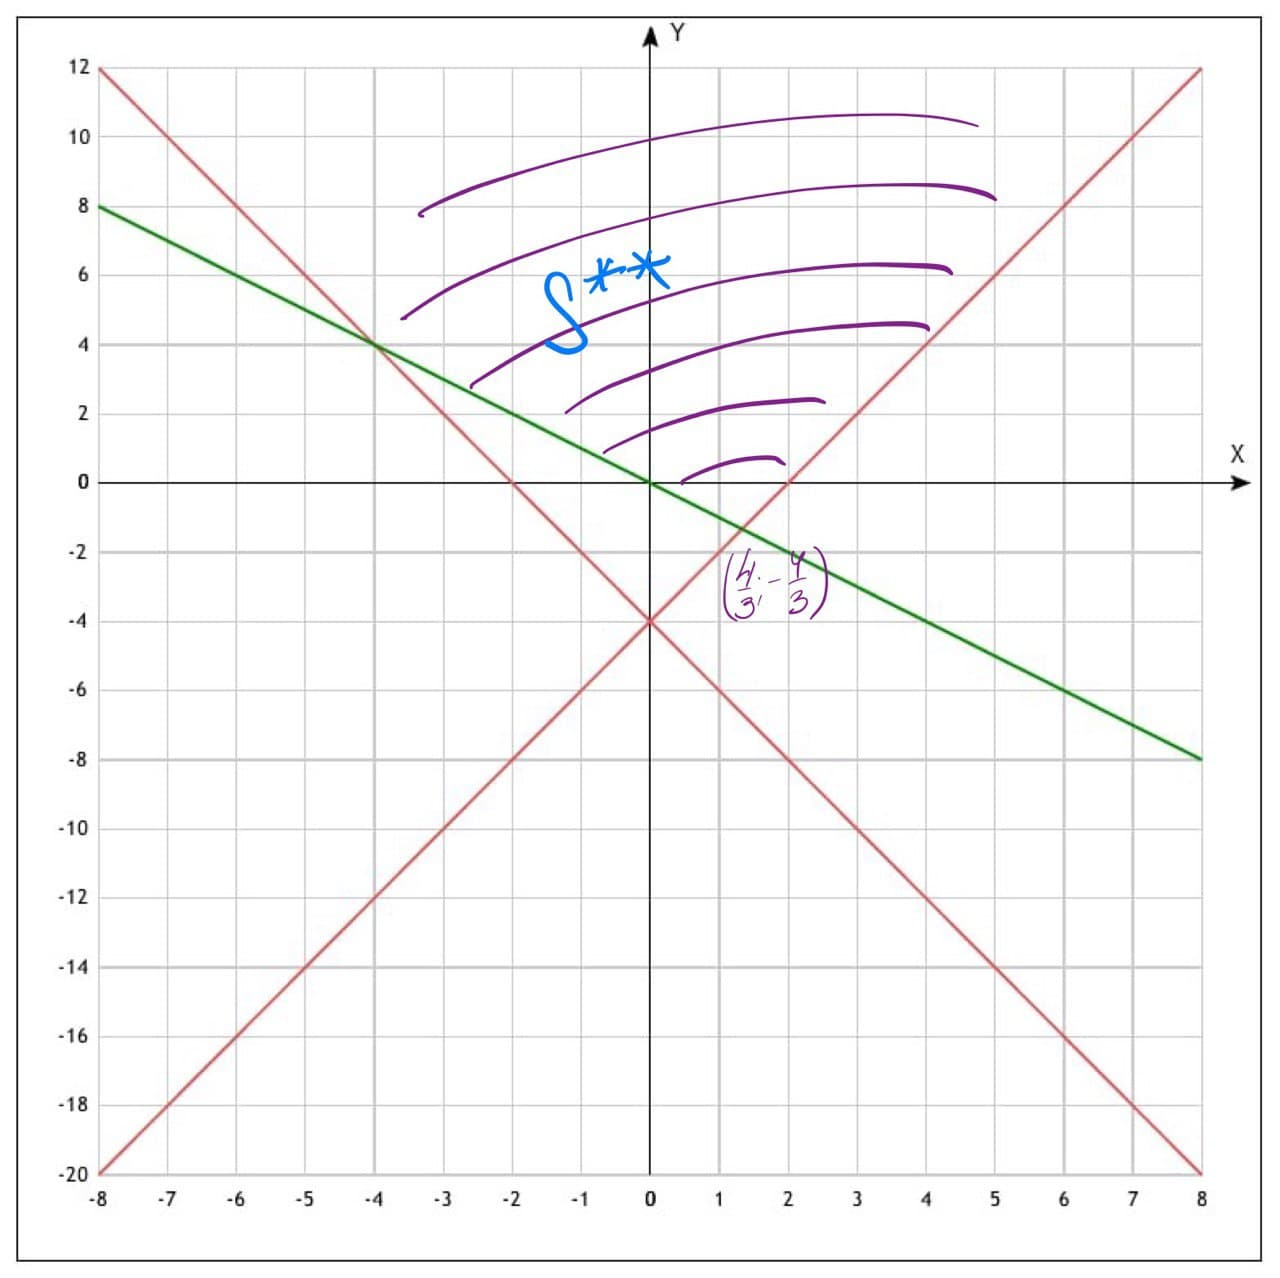
\includegraphics[width=0.6\linewidth]{S3}
\end{center}
\end{minipage}
\end{figure}

\newpage



\subsection*{Задача №4}
$\textbf{Find the conjugate cone for the exponential cone:}$
$$
K = \{(x, y, z) \mid y > 0, y e^{x/y} \leq z\}
$$

По определению, ищем вектора из $ \mathbb{R}^3 $ с коэффициентами $ (a, b, c) $ такие что: 
$$
(x, y, z)\left(\begin{array}{l}
a \\
b \\
c
\end{array}\right) \geq 0, \; \text{где}(x, y, z):\left\{\begin{array}{l}
y e^{x / y} \leq z \\
y>0
\end{array}\right.
$$

Замена: $ u = \frac{x}{y} $ и $ v = \frac{z}{y} $:
$$a u+b+c v \geq 0, \quad \text{где} \; (u, v): \left\{\begin{array}{l}
v>0 \\
v \geq e^{u}  \; 
\end{array}\right. $$ 
$ K^* $ - конус, рассматриваем 3 случая: $ c = -1 $, $ c = 0 $, $ c = 1 $, так как любой другой можно получить домножив на положительную константу, что не изменит результатов.

\begin{itemize}
	\item[c = 1: ] Выбираем a,b, чтобы в $ v \geq -au - b $ лежали все значения $v \geq e^{u}$.
	$$
\begin{aligned}
&\begin{array}{l}
a<0: \quad b \geq a(1-\ln (-a)) \\
a=0: \quad b \geq 0
\end{array}\\
&a>0: \text { нет подходящих } b
\end{aligned}
$$
\begin{figure}[h!]
\begin{minipage}[h]{1\linewidth}
\begin{center}
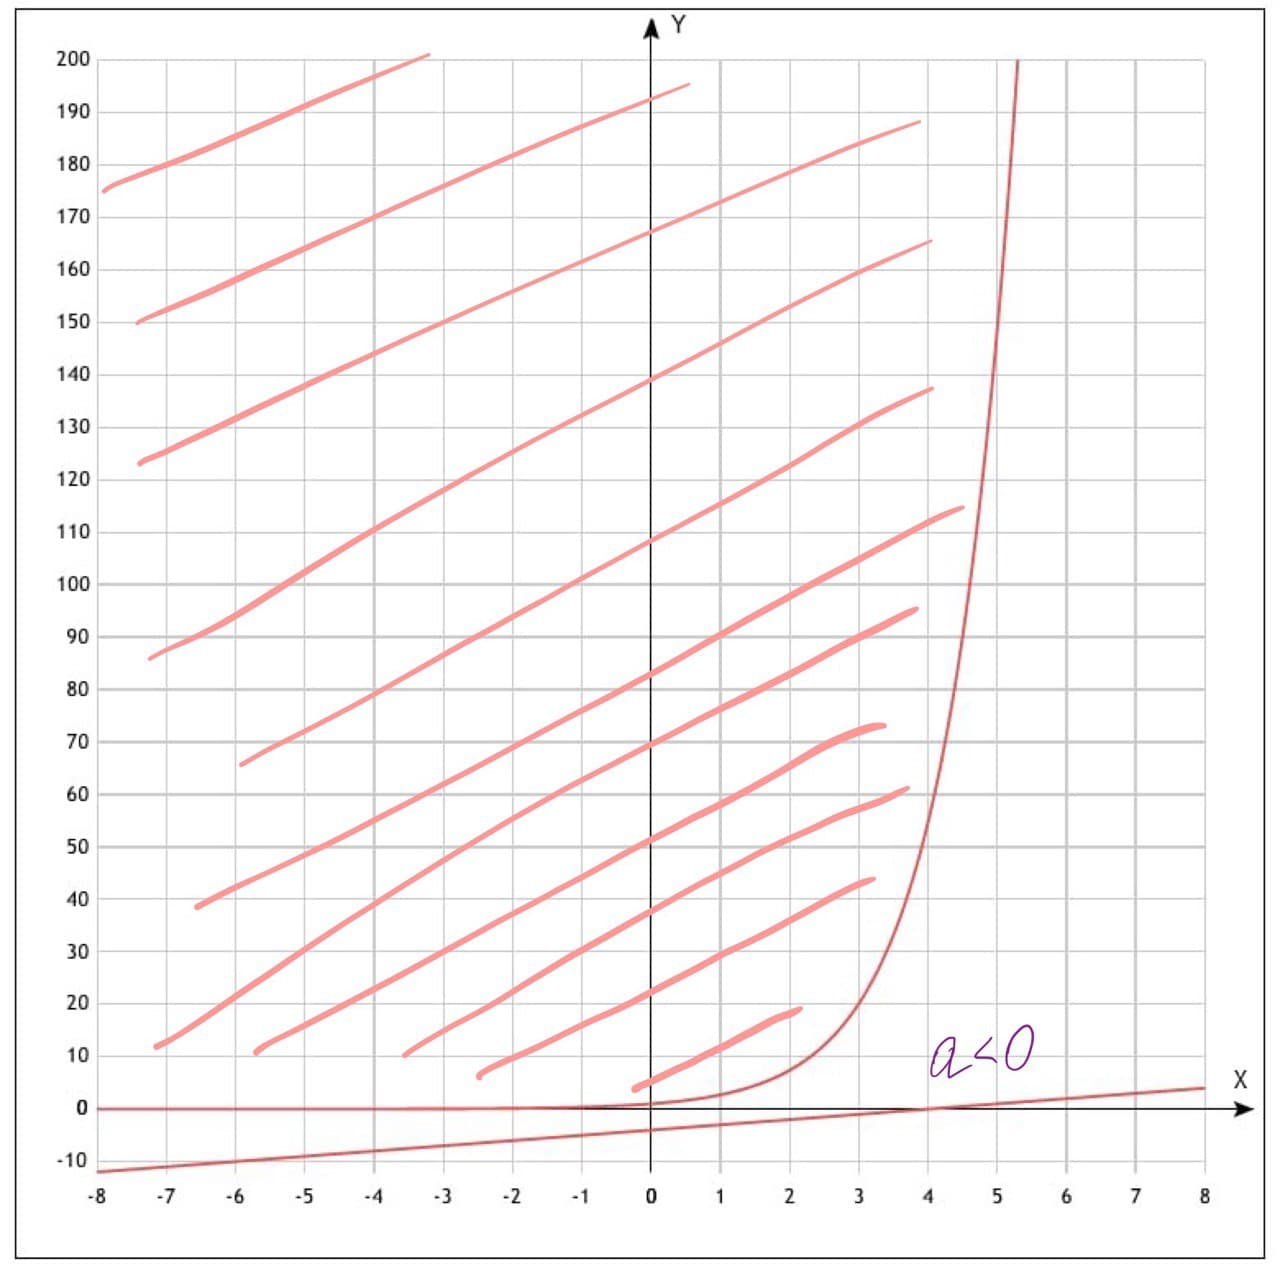
\includegraphics[width=0.6\linewidth]{cone}
\end{center}
\end{minipage}
\end{figure}
	
	\item[c = 0: ] В области $ au+b \geq 0 $ лежат все точки $v \geq e^{u}$, но таких a,b нет ($ au+b = 0 $ - вертикальная прямая).
	\item[c = -1: ] Множество точек  $v \geq e^{u}$ должно лежать выше прямой $ au+b \geq v $, но таких a,b нет (видно из графика).
\end{itemize}

$$
K^{*}=\left\{ \alpha \cdot (a, b, 1) \mid \alpha \geq 0, \begin{array}{l}
\text { при } a=0, \text { и } b \geq 0 \\
\text { при } a<0, \text { и } b \geq a(1-\ln (-a))
\end{array}\right\}
$$


\subsection*{Задача №5}
$\textbf{Prove, that}\ B_p, B_{p_*}\ \textbf{are inter-conjugate, i.e} (B_p)^*=B_{p_*}, (B_{p_*})^*=B_p,\ \textbf{where}\ B_{p}\\ \textbf{is the unit ball (w.r.t. p- norm) and}\ p,p_*\ \textbf{are conjugated, i.e.}\ p^{-1}+p^{-1}_*=1.\\ \textbf{You can assume, that}\ p_*=\infty, p=1\ \textbf{and vice versa.} $
\\Единичный шар $B:=\{x \in V: \parallel x\parallel<1\}$, является выпуклым, симметричным по x, замкнутым, норму можно записать как:
$$\parallel x\parallel=(sup\{t\geq0\mid tx\in B\})^{-1}$$
Из свойств сопряженной нормы:
$$({\parallel x \parallel}_p)_*={\parallel x \parallel}_{p_*},\ \text{if}\ \frac{1}{p}+\frac{1}{p_*}=1$$
У нас не бесконечномерное пространство => должно выполняться, ${\parallel x\parallel}_{**}=\parallel x\parallel,\ \forall x$

\newpage
\section{Conjugate function}
\subsection*{Задача №1}
$\textbf{Find}$ $f^*(y)$, if $f(x) = -\dfrac{1}{x}, \;\; x\in \mathbb{R}_{++}$\\

По определению сопряжённой функции: 
$$
f^*(y) = \sup_x \left( xy - f(x) \right) = \sup_x \left( xy + \frac{1}{x} \right) = \sup_x f(x,y)
$$

Область определения $ f^*(y) $ (при каких $ y $, $ \sup\limits_x \left( xy + \frac{1}{x} \right) $ - ограничен):
\begin{itemize}
	\item[1) ] если $ y > 0 $, то при $ x \rightarrow +\infty $, $ xy \rightarrow +\infty$, а $ \frac{1}{x} \rightarrow 0 $, следовательно $ f(x,y) \rightarrow +\infty $
	\item[2) ] если $ y < 0 $, то при $ x \rightarrow -\infty $, $ xy \rightarrow +\infty$, а $ \frac{1}{x} \rightarrow 0 $, следовательно $ f(x,y) \rightarrow +\infty $
	\item[3) ] если $ y = 0 $, то $ \forall x \; xy =0   $. При $ x \rightarrow 0 $, то $ \frac{1}{x} \rightarrow + \infty $, следовательно, $ f(x,y) \rightarrow +\infty $
\end{itemize}
Ответ: $ f^*(y) = +\infty $

\subsection*{Задача №2}
$\textbf{Prove, that if}\ f(x_1,x_2)=g_1(x_1)+g_2(x_2), \textbf{then}\ f^*(y_1,y_2)=g^*_1(y_1)+g^*_2(y_2)$

По определению сопряжённой функции: 
$$
\begin{aligned}
f^*(y_1,y_2)&=g^*_1(y_1)+g^*_2(y_2)= sup_{x_1}\{x^T_1y_1-g_1(x_1)\}+sup_{x_2}\{x^T_2y_2-g_2(x_2)\}=\\
&=sup_{x_1,x_2}\{x^T_1y_1-g_1(x_1)+x^T_2y_2-g_2(x_2)\}=sup_{x_1,x_2}\{x^T_1y_1+x^T_2y_2-f(x_1,x_2)\}
\end{aligned}
$$

\subsection*{Задача №3}
$\textbf{Find}$ $f^* (y)$, if $ f(x) = \log \left( \sum\limits_{i=1}^n e^{x_i} \right) $ \\

По определению сопряжённой функции: 
$$
f^{*}(y)=\sup _{x \in \operatorname{dom} f}(\langle y, x\rangle-f(x))
$$
Берем градиент: 
$$
y_{i}=\frac{e^{x_{i}}}{\sum_{j=1}^{n} e^{x_{j}}}, \quad i=1, \ldots, n
$$
Будем использовать определение двойственной функции:
$$
f^*(y) = \sum\limits_{i=1}^n y_i x_i - \log \left( \sum\limits_{i=1}^n e^{x_i} \right) = \sum\limits_{i=1}^n \log e^{x_i y_i} - \log \left( \sum\limits_{i=1}^n e^{x_i} \right) = \sum\limits_{i=1}^n
 \log  \frac {e^{x_i} e^{y_i} }{ \sum\limits_{i=1}^n e^{x_i} } = \sum\limits_{i=1}^n y_i \log y_i
$$

$ f^*(y_i) = y_i \log y_i $ - кросс-энтропия ($y \succ 0 \text { and } \mathbf{1}^{T} y=1$, $ y $ - вектор вероятности: все $ y_i > 0 $ и $ \sum \limits_{i = 1}^n y_i = 1 $  ). \\
Область определения: 
\begin{itemize}
\item[1)] Пусть существует компонента вектора $ y $, такая что $ y_i < 0 $. Возьмём вектор $x_{k}=-t, \text { и } x_{i}=0, i \neq k, t\rightarrow \infty$. Тогда $$ y^{T} x-f(x) \rightarrow\infty$$ как $ t - \log t $ => $ f^*(y) $ - неограничена. 
\item[2)] $ \text { Если } y \succeq 0 \text { но } \mathbf{1}^{T} y \neq 1, \text { выберем } x=t \mathbf{1}$
$$
y^{T} x-f(x)=t \mathbf{1}^{T} y-t-\log n
$$
\begin{itemize}
	\item[2.1)] $ \mathbf{1}^{T} y > 1 $ => $ f^*(y) $ - неограничена при $ t \rightarrow \infty $
	\item[2.2)] $ \mathbf{1}^{T} y < 1 $ =>  $ f^*(y) $ - неограничена при $ t \rightarrow -\infty $
\end{itemize}
\end{itemize}

$$
f^{*}(y)=\left\{\begin{array}{ll}
\sum_{i=1}^{n} y_{i} \log y_{i} & \text { если } y \succeq 0 \text { и } \mathbf{1}^{T} y=1 \\
\infty & \text { иначе }
\end{array}\right.
$$

\subsection*{Задача №4}
$\textbf{Prove, that if}$ $f(x) = \alpha g(x)$, then $f^*(y) = \alpha g^*(y/\alpha)$\\

По определению сопряжённой функции: 
$$
\begin{aligned}
f^{*}(y) &=\sup _{x} (x y-f(x))=\sup _{x}(x y-\alpha g(x))=\\
&=\sup _{x} \left(\alpha\left[x \cdot \frac{y}{\alpha}-g(x)\right]\right)=\alpha \sup _{x, \alpha>0} \left(x \cdot \frac{y}{\alpha}-g(x)\right) =\\
&= \alpha \cdot g^* \left( \frac{y}{\alpha} \right)
\end{aligned}
$$

\subsection*{Задача №5}
$\textbf{Find}$ $f^*(Y)$, if $f(X) = - \ln \det X, X \in \mathbb{S}^n_{++}$\\
По определению сопряжённой функции: 
$$
f^{*}(Y)=\sup _{X \succ 0}(\operatorname{tr}(Y^T X)+\log \operatorname{det} X)
$$
используем $ \operatorname{tr}(Y^T X) $ как операцию скалярного умножения на матрицах. $ f^{*}(Y) $ неограничена, если $ Y \nprec 0 $ ($ Y $ имеет собственный вектор $ v $ с $ \lambda \geq  0 $ и без ограничения общности $ \|v\|_{2}=1 $), тогда возьмём $ X=I+t v v^{T} $, получим: 
$$
\operatorname{tr}(Y^T X)+\log \operatorname{det} X=\operatorname{tr} Y^T+t \lambda+\log \operatorname{det}\left(I+t v v^{T}\right)=\operatorname{tr} Y^T+t \lambda+\log (1+t)
$$
Неограничено при $ t \rightarrow \infty $.\\
Если $ Y \prec 0 $, найдём максимум:
$$
\nabla_{X}(\operatorname{tr}(Y^T X)+\log \operatorname{det} X)=Y+X^{-1}=0
$$
$ X = -Y^{-1} $ ($ X $ - положительно определена, симметричная => $ Y $ симметричная). По определению:
$$
f^{*}(Y)=\log \operatorname{det}(-Y)^{-1}-n
$$
область определения: $ \operatorname{dom} f^{*}=-\mathbb{S}_{++}^{n} $

\subsection*{Задача №6}
$\textbf{Prove, that if}\ f(x) = inf_{u+v=x}(g(u)+h(v)), \textbf{then}\ f^*(y)=g^*(y)+h^*(y)$

Запишем по определению:
$$f^*(y)= sup_x\{<x,y>-f(x)\}$$
Тогда можем подставить нашу f(x):
$$f^*(y)= sup_x\{<x,y>-inf(g(u)+h(v))\mid u+v = x\}$$
Упрощаем:
$$
\begin{aligned}
f^*(y)&= sup_{x,u,v}\{x^Ty-g(u)-h(v)\mid u+v=x\}=sup_{u,v}\{(u+v)^Ty-g(u)-h(v)\}=\\
&= sup_u\{u^Ty-g(u)\}+sup_v\{v^Ty-h(v)\}=g^*(y)+h^*(y)
\end{aligned}
$$


\newpage
\section{Subgradient and subdifferential}

\subsection*{Задача 1}
$\textbf{Prove, that}$ $x_0$ $\textbf{- is the minimum point of a convex function}$ $f(x)$ $\textbf{if and only if}$ $0 \in \partial f(x_0)$\\

По определению $ g $ - субградиент $ f(x) : S\rightarrow R $ в точке $ x_0 $, если $ \forall x \in S $
$$
f(x) \geq f\left(x_{0}\right)+\left\langle g, x-x_{0}\right\rangle
$$
Множество всех субградиентов $ f(x) $ в точке $ x_0 $ - субдифференциал $ f $ в $ x_0 $. 
$$ 0 \in \partial f(x_0) \longrightarrow f(x) \geq f\left(x_{0}\right), \quad \forall x \in S $$
Получаем определение минимума выпуклой функции => утверждения эквивалентны.

\subsection*{Задача 2}
$\textbf{Find}$ $\partial f(x)$, if $f(x) = \text{ReLU}(x) = \max \{0, x\}$\\

По теореме Дубовитского-Милютина ($ 0 $ и $ x $ - выпуклые функции на выпуклом множестве $S \subseteq \mathbb{R}^{n} $): 
$$
\begin{array}{r}
\partial_{S} f\left(x_{0}\right)=\operatorname{conv}\left\{\bigcup\limits_{i \in I\left(x_{0}\right)} \partial_{S} f_{i}\left(x_{0}\right)\right\} \\
\end{array}
$$
где $I(x)=\left\{i \in[1: m]: f_{i}(x)=f(x)\right\}$
\begin{itemize}
	\item[$ x > 0 $ ] - активная функция $ y = x $
	\item[$ x < 0 $] - активная функция $ 0 $
	\item[$ x = 0 $] - обе функции активны, берём выпуклую оболочку
\end{itemize}

$$
\partial f(x)=\left\{\begin{array}{l}
1, \quad x>0 \\
\{0\}, \quad x<0 \\
\left\{a \mid a=\lambda a^{\prime}, 0 \leq \lambda \leq 1, a^{\prime} \in \partial x = 1 \right\}, \quad x=0
\end{array}\right.
$$

\subsection*{Задача 3}
$\textbf{Find}$ $\partial f(x)$, if $f(x) = \|x\|_p$ $\textbf{при}$ $p = 1,2, \infty$\\

\begin{itemize}
	\item[1. ] $ f(x) = \| x \|_1 $, по определению:
	$$
\|x\|_{1}=\left|x_{1}\right|+\left|x_{2}\right|+\ldots+\left|x_{n}\right|=s_{1} x_{1}+s_{2} x_{2}+\ldots+s_{n} x_{n}
$$
где $ s_i = \{ -1, 1 \} $\\
Можно рассмотреть как поточечный максимум линейных функций, по теореме Дубовицкого-Милютина в каждой точке:
$$
\partial f=\operatorname{conv}\left(\bigcup_{i \in I\left(x\right)} \partial g_{i}(x)\right)
$$
где $ \partial g_i(x) = \nabla g_i(x) = s_i $ (линейность):

$$
\partial g(x)=\partial\left(\max \left\{s^{\top} x,-s^{\top} x\right\}\right)=\left\{\begin{array}{ll}
-s, & s^{\top} x<0 \\
\operatorname{conv}(-s ; s), & s^{\top} x=0 \\
s, & s^{\top} x>0
\end{array}\right.
$$

\begin{itemize}
\item[1) ]  Если j-ая координата точки отрицательна, $s_i^j = -1$
\item[2) ] Если j-ая координата точки положительна, $s_i^j = 1$
\item[3) ] Если j-ая координата точки равна нулю, субградиенты этих функций включены в объединение в теореме Дубовицкого - Милютина
\end{itemize}

$$
\partial f(x)=\left\{g:\|g\|_{\infty} \leq 1, \quad g^{\top} x=\|x\|_{1}\right\}
$$


	\item[2. ] По определению:
$$
\|x\|_{2}= \sqrt{\sum\limits_{i=1}^n x_i^2} 
$$ 
Функция дифференцируема во всех точках, кроме $0_n$ => если $x\neq0_n$:
$$
\partial f(x) = \nabla (\|x\|_{2}) = \frac{\textbf{x} }{\| x \|_2} 
$$
Для $0_n$:
$$f(0_n, p)=lim _{\alpha\rightarrow0+}\frac{{\parallel\alpha p\parallel}_2}{\alpha}={\parallel p\parallel}_2$$
Опорная функция единичного шара => $$\partial f(0_n)=\{x\mid{\parallel x\parallel}_2\leqslant1\}.$$

	\item[3. ] По определению:
$$
f(x) = \| x \|_{\infty} = \max\limits_i |x_i|
$$
По теореме Дубовитского-Милютина о поточечном максимуме ($ |x_i| $ - выпуклые функции):
$$
\partial f(x) = \operatorname{conv}\left\{\bigcup_{i \in I\left(x\right)} \partial |x_i| \right\}
$$
где $
I(x)=\left\{i \in[1: m]: f(x)=|x_i|\right\}
$\\
Субдифференциал для модуля $ x $:
$$
\partial\left|x_{i}\right|=\left\{\begin{array}{l}
\operatorname{sign}\left(x_{i}\right), x_i \neq 0 \\
{[-1,1], x_i=0}
\end{array}\right.
$$

Получается, 
$$
\partial f(x) = \left\{\begin{array}{l}
\operatorname{sign}\left(x_{i}\right), x_i \neq 0 \\
{[-1,1], x_i=0}
\end{array}\right.
$$
где $ x_i $ - максимальный элемент в векторе
\end{itemize}
 

\subsection*{Задача 4}
$\textbf{Find}$ $\partial f(x)$, if $f(x) = \|Ax - b\|_1$\\

Пусть $ g(x) = \|x\|_1 $ - выпуклая функция, тогда $ f(x) = \|Ax - b\|_1 = g(Ax-b) $.\\
Так как $ g(x) $ - выпуклая функция, то можем применить свойство субдифференциального исчисления: 
$$ \partial f(x) = \partial(g(A x+b))(x)=A^{T} \partial g(A x+b) $$ 
$$ \partial g(x) = \partial \|x\|_1 = \{ \phi : \|\phi\|_{\infty} \leq 1, \phi^T x = \|x\|_1 \} $$
$$ \partial f(x) = A^{T} \cdot \{ \phi : \|\phi\|_{\infty} \leq 1, \phi^T (Ax + b) = \|Ax + b\|_1 \} $$

\subsection*{Задача 5}
$\textbf{Find}$ $\partial f(x)$, if $f(x) = e^{\|x\|}$\\

Рассматриваем, как сложную функцию от $ g(x) = \|x\|_p $, для которой субдифференциал мы нашли в задаче 3.\\
Возведение в экспоненту монотонно неубывающая функция, дифференцируемая, выпуклая. Операторная форма - выпуклая функция =>
$$\partial f(x) = e^{\|x\|_p} \cdot \partial \|x\|_p$$

\subsection*{Задача 6}
$
\textbf { Find } \partial f(x) \text { , if } f(x)=\max\limits _{i}\left\{\left\langle a_{i}, x\right\rangle+b_{i}\right\}, a_{i} \in \mathbb{R}^{n}, b_{i} \in \mathbb{R}, i=1, \ldots, m
$\\

Перепишем в виде: $ f_i = \left\{\left\langle a_{i}, x\right\rangle+b_{i}\right\} $, $ i=1, \ldots, m $. $ f(x) = \max\limits _{i = \overline{1,m}}\left\{ f_i \right\}$ - выпуклые функции на множестве $ S = \mathbb{R}^n $\\
Можем использовать теорему Дубовитского-Милютина:
$$
\begin{array}{l}
\partial_{S} f\left(x\right)=\operatorname{conv}\left\{\bigcup_{i \in I\left(x\right)} \partial_{S} f_{i}\left(x\right)\right\} \\
\end{array}
$$
$I(x)=\left\{i \in[1: m]: f_{i}(x)=f(x) - \text{активные индексы}\right\}$
$ f_i(x) $ - линейные функции и их субдифференциал равняется градиенту: 
$$
\partial_{S} f\left(x\right)=\operatorname{conv}\left\{\bigcup_{i \in I\left(x\right)} a_i\right\}
$$
где $ I(x)=\left\{i \in[1: m]: f(x)=f_{i}(x)= a_i x + b_i \right\} $
$$
\partial_{S} f\left(x\right) = \left(\sum_{i \in I(x)} \lambda_{i} a_{i}: \sum_{i \in I(x)} \lambda_{i}=1, \quad \lambda_{i} \geq 0, i \in I(x)\right)
$$
где $ I(x)=\left\{i \in[1: m]: f(x)= a_i x + b_i \right\} $


\end{document}
